\documentclass{standalone}
\usepackage{tikz}
\begin{document}
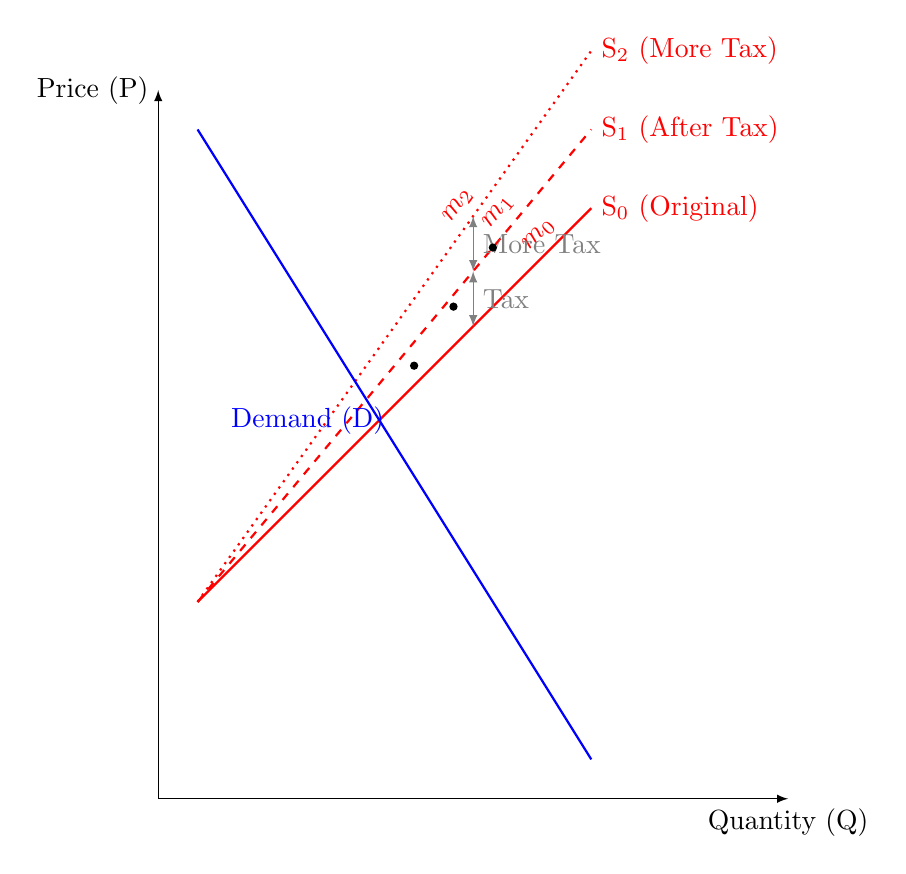
\begin{tikzpicture}[scale=1, >=latex]
    % Axes with padding
    \draw[->] (0,0) -- (8,0) node[below] {Quantity (Q)};
    \draw[->] (0,0) -- (0,9) node[left] {Price (P)};

    % Original supply point (hidden anchor)
    \coordinate (origin) at (0.5,2.5);

    % Supply curves with different slopes through (0.5,2.5)
    \draw[red, thick] (0.5,2.5) -- (5.5,7.5) node[right] {S\textsubscript{0} (Original)} 
        node[sloped, pos=0.9, above] {$m_0$};
    \draw[red, thick, dashed] (0.5,2.5) -- (5.5,8.5) node[right] {S\textsubscript{1} (After Tax)} 
        node[sloped, pos=0.8, above] {$m_1$};
    \draw[red, thick, dotted] (0.5,2.5) -- (5.5,9.5) node[right] {S\textsubscript{2} (More Tax)} 
        node[sloped, pos=0.7, above] {$m_2$};

    % Demand curve
    \draw[blue, thick] (0.5,8.5) -- (5.5,0.5) node[midway, above left] {Demand (D)};

    % Tax arrows at Q=4
    \draw[<->, gray] (4,6.0) -- node[midway, right] {Tax} (4,6.7);
    \draw[<->, gray] (4,6.7) -- node[midway, right] {More Tax} (4,7.4);

    % Equilibrium points (hidden)
    \fill[black] 
        (3.25,5.5) circle (1.5pt)  % S₀-D intersection
        (3.75,6.25) circle (1.5pt) % S₁-D intersection
        (4.25,7.0) circle (1.5pt); % S₂-D intersection
\end{tikzpicture}
\end{document}